\documentclass{homework}
\usepackage{tikz}
\usetikzlibrary{positioning,shapes,arrows}

\title{Assignment2: Bayesian Networks}
\author{
  Dmitrii, Maksimov\\
  \texttt{dmitrii.maksimov@fau.de} \\
  \texttt{ko65beyp}
  \and
  Ilia, Dudnik\\
  \texttt{ilia.dudnik@fau.de}\\
  \texttt{ex69ahum}
  \and
  Aleksandr, Korneev\\
  \texttt{aleksandr.korneev@fau.de}\\
  \texttt{uw44ylyz}
}
\begin{document}

\maketitle

\exercise[2.3 (Medical Bayesian Network 2)]

Both Malaria and Meningitis can cause a fever, which can be measured by
checking for a high body temperature. Of course you may also have a high body temperature for other reasons. We consider the following random variables for a given patient:
\begin{itemize}
	\item \emph{Mal}: The patient has malaria
	\item \emph{Men}: The patient has meningitis.
	\item \emph{HBT}: The patient has a high body temperature.
	\item \emph{F}: The patient has a fever.
\end{itemize}
\begin{enumerate}
	\item Draw the corresponding Bayesian network for the above data using the algorithm presented in the lecture, assuming the variable order $Mal,Men,HBT,F.$ Explain rigorously(!) the exact criterion for whether to insert an arrow between two nodes.
		\begin{center}
		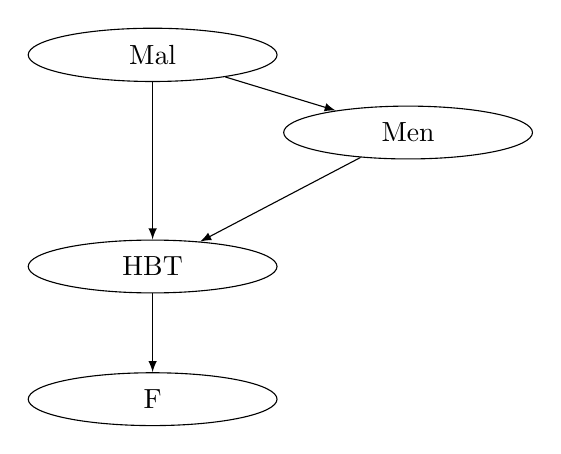
\begin{tikzpicture}[
		  node distance=1cm and 0cm,
		  mynode/.style={draw,ellipse,text width=2cm,align=center}
		]
		\node[mynode] (Mal) {Mal};
		\node[mynode, below right=0.5 cm and 1 cm of Mal] (Men) {Men};
		\node[mynode,below=2cm of Mal] (HBT) {HBT};
		\node[mynode,below=1cm of HBT] (F) {F};
		\path (Mal) edge[-latex] (Men)
			(Mal) edge[-latex] (HBT)
			(Men) edge[-latex] (HBT)
			(HBT) edge[-latex] (F);
		\end{tikzpicture}
		\end{center}
	\begin{itemize}
		\item $Mal$: $Men$ - assume that $Mal$ affects the $Men$; $HBT$ - affects by far; $F$ - given HBT, knowing $Mal$ doesn’t give any more information about F - no arrow.
		\item $Men$: $HBT$ - affects by far; $F$ - given HBT, knowing $Men$ doesn’t give any more information about F - no arrow.
		\item $HBT$: $F$ -  affects by far.
	\end{itemize}
	\item Which arrows are causal and which are diagnostic? Which order of variables would be better suited for constructing the network?
	
	$Mal \rightarrow HBT$ and $Men \rightarrow HBT$ are causal arrows. $HBT \rightarrow F$ is diagnostic arrow. Order $Mal, Men, F, HBT$ would be better because we wouldn't have to think about adding arrows like $Mal \rightarrow F$. Which in the proposed order were not added only because of common sense. However, the network would look the same, only $HBT$ and $F$ would be swapped.
	\item How do we compute the probability the patient has malaria, given that he has a fever? State the query variables, hidden variables and evidence and write down the equation for the probability we are interested in.
	
	Hidden variables: $Y = \{HBT, Men\}$\newline
	Query variables: $X = \{Mal\}$\newline
	Evidence variables: $E = \{F\}$\newline
	$ P(Mal|F) = \alpha P(Mal, F) = \alpha(\sum_{Men}\sum_{HBT} P(Mal, F, Men,HBT)) = \newline \alpha(\sum_{Men}\sum_{HBT} P(Mal)\cdot P(Men|Mal)\cdot P(HBT|Mal,Men)\cdot P(F|HBT))$, \newline where
	$\alpha = \dfrac{1}{P(F)}$
\end{enumerate}

\end{document}